\documentclass[12pt]{paper}
\usepackage[english]{babel}
\usepackage{indentfirst}
\usepackage{graphicx}
\usepackage{latexsym}
\usepackage{amsmath}
\usepackage{amsthm}
\usepackage{amssymb,amsfonts}
\usepackage{multicol}
\usepackage{xcolor}
\usepackage{changepage}
\usepackage{hyperref}
\usepackage{fancyhdr}
\usepackage{textcomp}
\usepackage{mathtools}
\usepackage{comment}
\usepackage[normalem]{ulem}
\usepackage{marginnote}
\usepackage[numbers,sort&compress]{natbib}
\mathtoolsset{showonlyrefs=false}

\newcommand{\ga}{\alpha}
\newcommand{\gb}{\beta}
\newcommand{\gam}{\gamma}
\newcommand{\gd}{\delta}
\newcommand{\eps}{\epsilon}
\newcommand{\veps}{\varepsilon}
\newcommand{\gz}{\zeta}
\newcommand{\gt}{\theta}
\newcommand{\gi}{\iota}
\newcommand{\gk}{\kappa}
\newcommand{\gl}{\lambda}
\newcommand{\gs}{\sigma}
\newcommand{\go}{\omega}
\newcommand{\Gam}{\Gamma}
\newcommand{\gD}{\Delta}
\newcommand{\gT}{\Theta}
\newcommand{\gL}{\Lambda}
\newcommand{\gS}{\Sigma}
\newcommand{\gO}{\Omega}

%%%%%%%%%

\newcommand{\pt}[1]{\left( #1\right)}
\newcommand{\pq}[1]{\left[ #1 \right]}
\newcommand{\pg}[1]{\left\{ #1\right\}}
\newcommand{\figref}[1]{\figurename~\ref{#1}}
\newcommand{\red}[1]{\textcolor{red}{#1}}
\newcommand{\blue}[1]{\textcolor{blue}{#1}}
\newcommand{\gray}[1]{\textcolor{gray}{#1}}
\newcommand{\wikilink}[2] { \href{#1.pdf}{#2}\,(\href{#1.tex}{edit})}

\setlength{\textheight}{20cm}
\changepage{3.4cm}{5cm}{-2cm}{-2.5cm}{-2.0cm}{-2cm}{0.3cm}{-0.5cm}{0.1cm}
%{length of the text}{width of the text}{}{shift to the right}
%{}{}{}{}{from text to pagenumber}
\pagestyle{fancy}
\lhead{\bf \today}
\chead{\bf }
\rhead{EG}
\title{Two polymers -- \today}
\author{EG}
\date{\today}

\begin{document}
 \maketitle
\wikilink{home}{Home}

\wikilink{twoPolymers}{Self}
% % Remove brackets from numbering in List of References
% \makeatletter
% %\renewcommand{\@biblabel}[1]{\quad#1.}
% \makeatother
% \renewcommand{\indexname}{Notations}
% \renewcommand{\familydefault}{\sfdefault}


 \begin{center}
  {\Large \textbf{Two polymers instead of two}}
 \end{center}
Ken believes 1 polymer isn't capable of generating life.
instead we need 2 -- functional, which gets destroyed quickly and informational, which is more 
stable.

\begin{itemize}
 \item Legend to Petri Nets diagrams, which I'm using here
\begin{figure}[h!]
 \centering
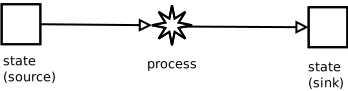
\includegraphics[width=0.35\textwidth]{pictures/legend.png}
\end{figure}
\item Good. (Machines get destroyed faster than Blueprints)
\begin{figure}[h!]
 \centering
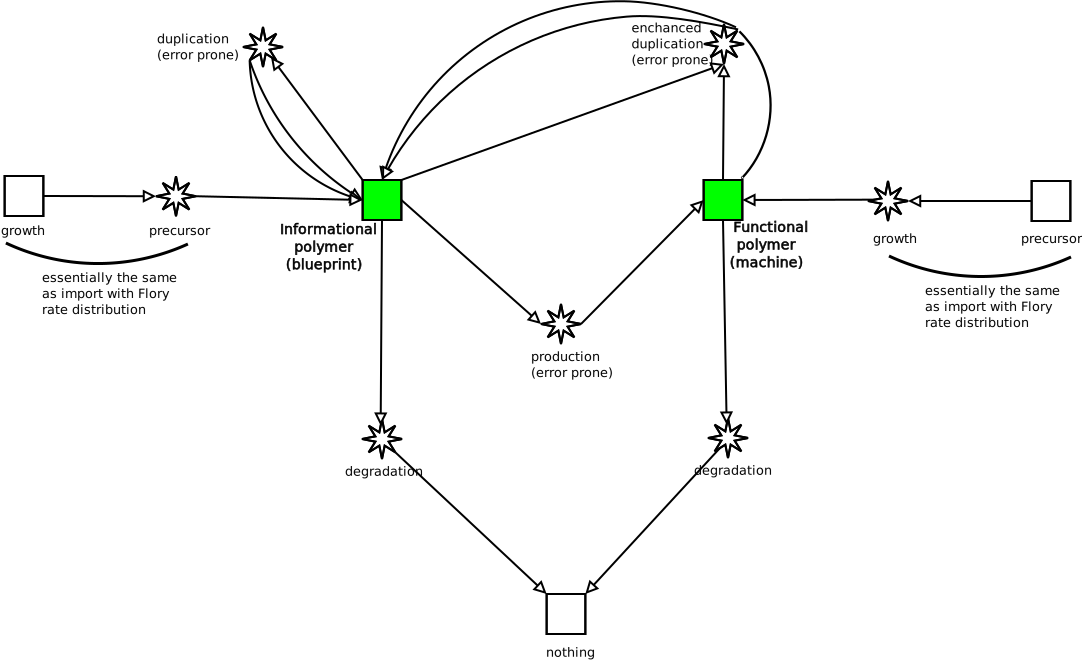
\includegraphics[width=0.89\textwidth]{pictures/blueprint-machine.pdf}
\end{figure}

\item Bad. 
\begin{figure}[h!]
 \centering
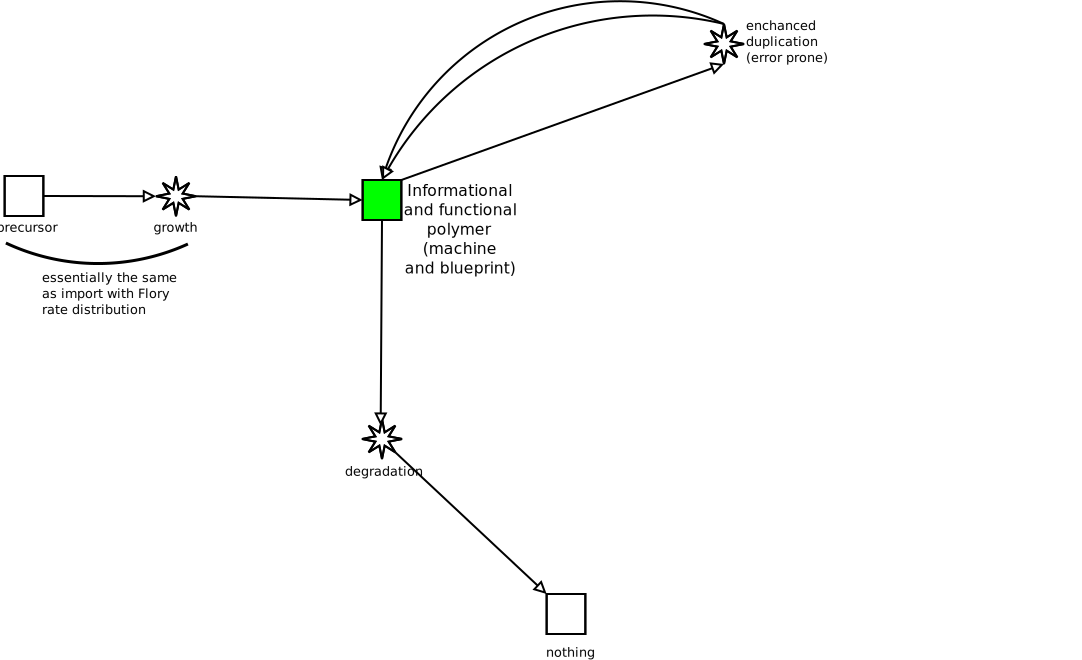
\includegraphics[width=0.69\textwidth]{pictures/selfreplicating-machine.pdf}
\end{figure}
\end{itemize}

\newpage
\section{New approach}
\begin{itemize}
 \item 
We have two types of polymers: memory polymer and function polymer. 
\item They are located inside little 
droplets. 
\item Different droplets have different sequences. Therefore those sequences vary in efficiency of
whatever they are doing.
\item Whenever a droplet gets a couple of functional sequences, the growth of the droplet starts and
essentially it splits into two daughter cells
\item Functional polymers get recycled faster. But Informational polymers live longer.
\red{Oops!! We don't have degradation in our model. Things are getting awfully complicated.}
\item Each time a new sequence is being produced on the basis of an old one, mistakes can be made. 
Number of mistakes has its distribution; either Gauss or Poisson.  
\item If the mapping memory-function is too broad, then we end up producing random sequences, and 
cells stop propagating efficiently. However, if we are lucky, then cells happen to win. \red{Lucky 
in what??}
\item The output number in number of copies of cells of a given cell type. The more -- the better.
\end{itemize}

\begin{figure}[h!]
 \centering
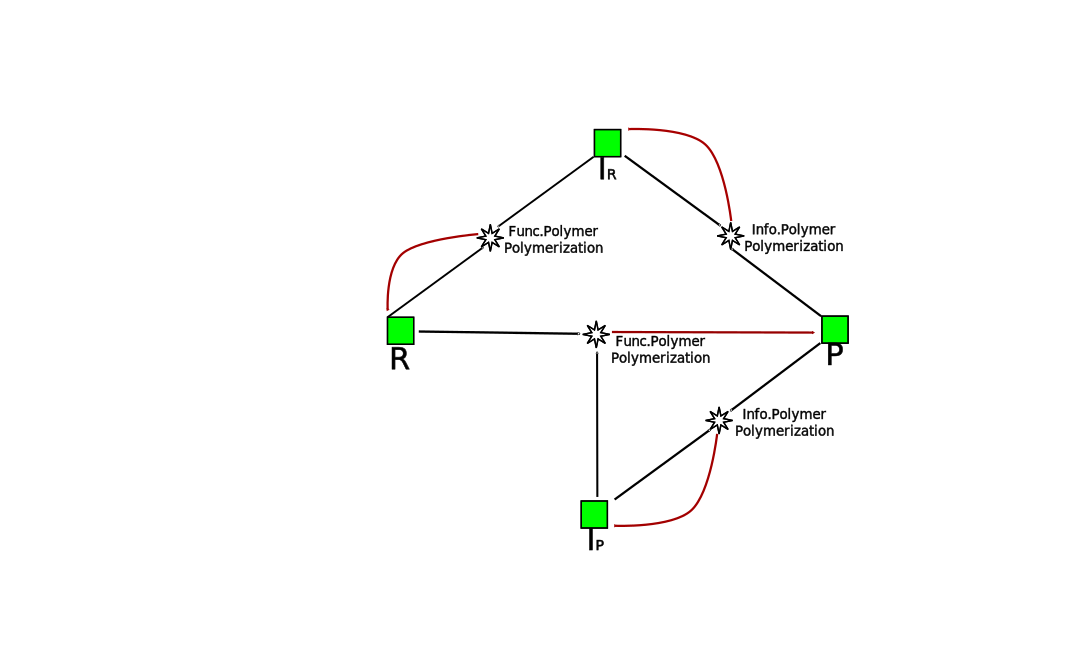
\includegraphics[width=0.59\textwidth]{pictures/info-func-porymers-newview.pdf}
\end{figure}

\section{Notes from Kinematic Self-Replicating Machines \cite{Freitas2004}}
\begin{itemize}
 \item 
\end{itemize}


 \bibliography{/data/research/31.mendeleyBibtex/library}
\end{document}
